\begin{section}[]{\uppercase{Methodology}}
 \addtocontents{toc}{\uppercase{Methodology}}
 Deepfake detection has become a crucial part of the digital world. 
 The research has been conducted to detect deepfakes using Deep Learning in various fields, especially in detection and recognition. 
 From medical imaging, disease detections and classifications to sentiment analysis. 
 Image recognition has created huge hype in field of DL. Many approaches like LSTM (Long Short-Term Memory), convolutional traces, GANs (Generative Adversarial Networks) are used for the deepfakes detection. Targeting specific features sets limitation as they can sometimes miss vital points.
 For this research combined approach is opted. Research began with the primary research by consulting the expertise regarding the topic and research questions. 
 Then alongside it, Literature Reviews, observation played a vital role for the research to take its shape. 
 Since plethora of research works have been carried out in this field, to review the previous research works and their findings to gain broad and better understanding of the subject was vital, it was resourceful and helped in identifying the research gap.

 \subsection{Dataset Description}
  The dataset used for this research is from the open-source website Kaggle \cite{Kaggle140kFaces}. The dataset consists of fake and real face images. The dataset is divided into training, validation and testing sets. The model will be trained on training set and validated on validation set. The model will be tested on testing set and the results will be evaluated using accuracy, F1-score, precision and recall. The results will be compared with other models and the proposed model will be evaluated. The dataset consists of 140,000 images of faces. 
  The dataset is divided into 70,000 images of fake faces and 70,000 images of real faces. Fake images were generated using NVIDIA's Style-Based Generator Architecture.
  Dataset from: https://www.kaggle.com/code/dima806/deepfake-vs-real-faces-detection-vit/input
  
  \par Figure \ref{fig:fake-real-faces} shows the fake and real faces from the dataset.
  
  \begin{figure}
    \centering
    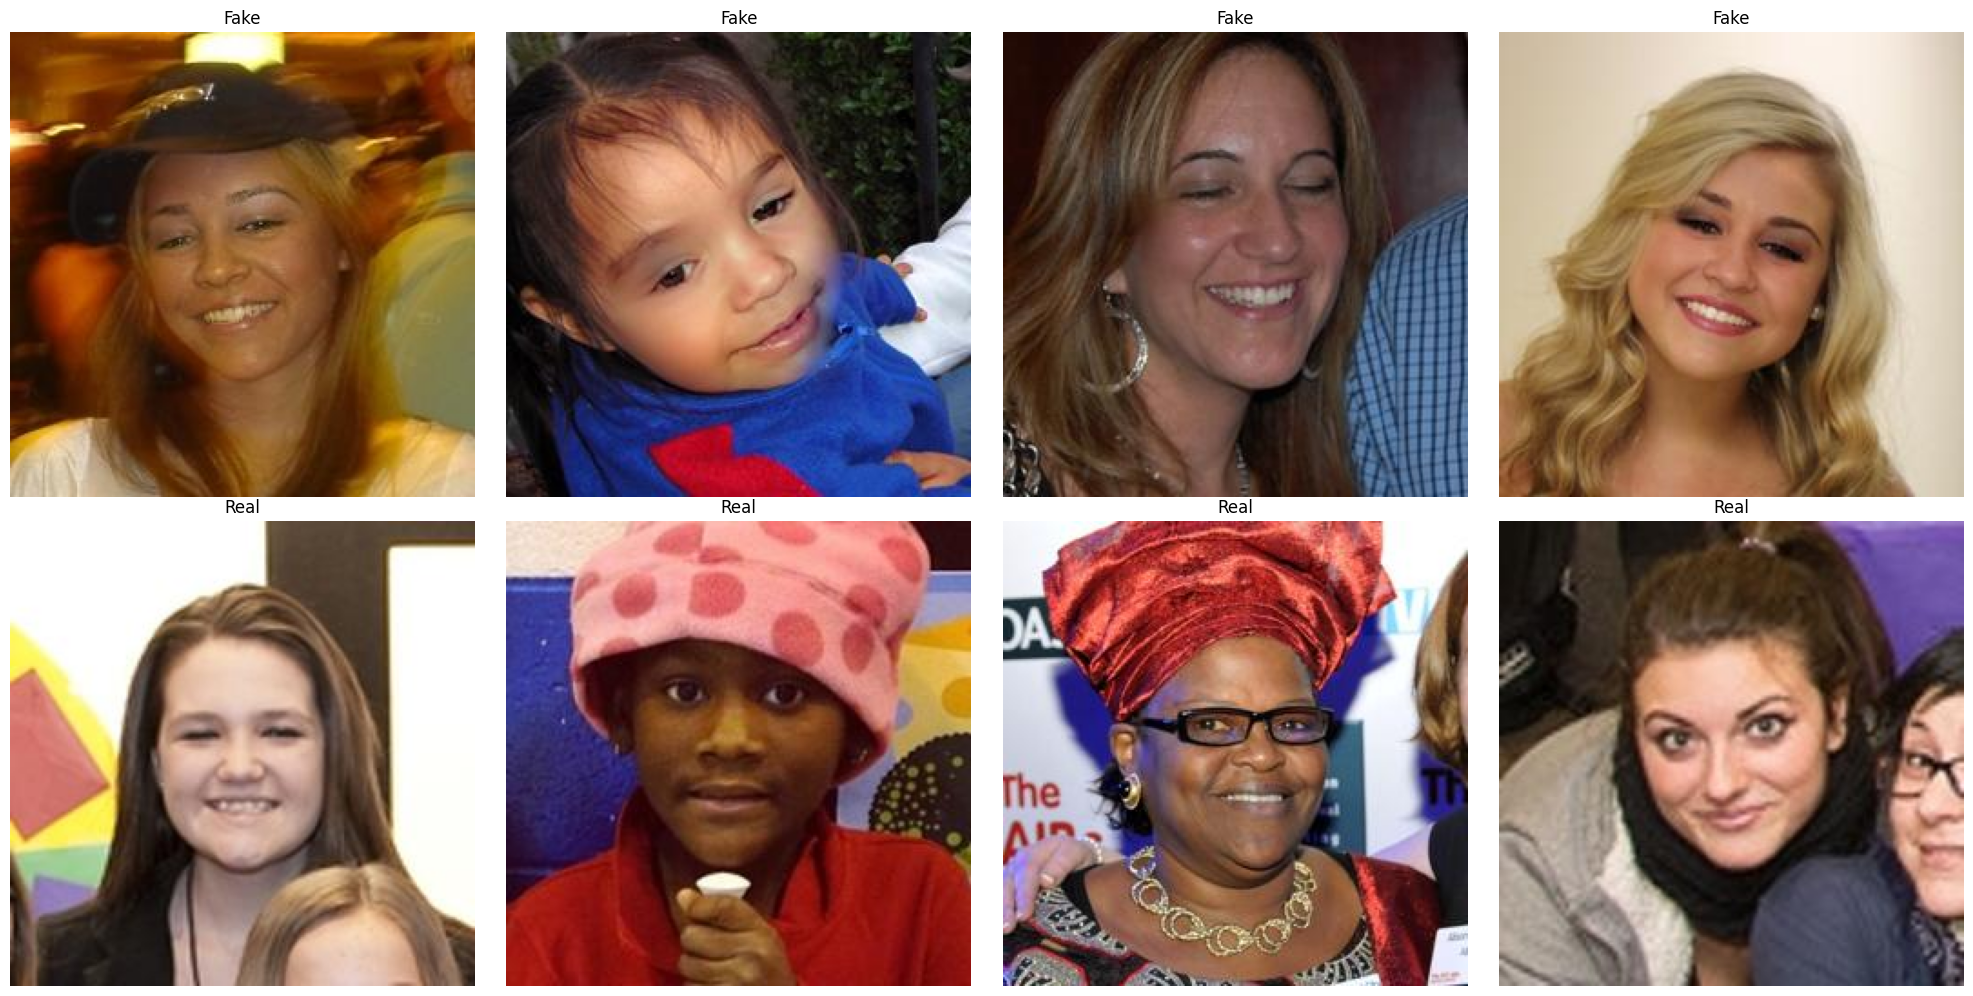
\includegraphics[width=\linewidth]{images/datasets.png}
    \caption{Fake and Real faces}
    \label{fig:fake-real-faces}
 \end{figure}
 
 \subsection{Development of Proposed Model}

 \begin{enumerate}
    \item \textbf{Python using Keras}: As the primary programming language, due to its robust support for data analysis and machine learning libraries.
    \item \textbf{TensorFlow}: These are the leading machine learning frameworks that are used for developing and training AI models, particularly for their support in building and deploying complex neural networks like LSTM.
\end{enumerate}

The model is develop in Google Colab, a cloud-based platform that is short for Google Colaboratory, is a platform offered free of charge by Google that lets you write and run python code in your browser. In particular, it lets you run Jupyter notebooks without having to worry about your hardware or the software installed on your computer. \cite{DataScientest2021}
Google Colab is a tool that also facilitates access to computing resources and common machine learning libraries. 

 \subsubsection{Proposed DICNN Model}
To develop the model with same trainable params as developed in the base research paper \cite{Bhandari2023}, it was developed in python using Keras and TensorFlow framework. Images were split into train, test and validation sets after preprocessing. Same layers and architecture are used as in the base research paper to test the validity of the model as documented in the paper. The model is then trained with with better optimizer and different datasets to test it's efficiency.

 \begin{table}[htbp]
    \centering
    \begin{tabular}{>{\raggedright\arraybackslash}p{4cm} >{\raggedright\arraybackslash}p{4cm} r >{\raggedright\arraybackslash}p{3cm}}
        \toprule
        \textbf{Layer Name} & \textbf{Shape of Output} & \textbf{Param \#} & \textbf{Connected to} \\
        \midrule
        Input 1 & (None, 224, 224, 3) & 0 & - \\
        Input 2 & (None, 224, 224, 3) & 0 & - \\
        Conv2D & (None, 222, 222, 32) & 896 & Input 1 \\
        Flatten 1 & (None, 150,528) & 0 & Input 2 \\
        Flatten 2 & (None, 1,577,088) & 0 & Conv2D \\
        Concatenate Layer & (None, 1,727,616) & 0 & [Flatten 1, Flatten 2] \\
        Dense 1 & (None, 224) & 386,986,208 & Concatenate Layer \\
        Dropout & (None, 224) & (None, 224) & Dense 1 \\
        Dense 2 & (None, 2) & 450 & Dropout \\
        \bottomrule
    \end{tabular}
    \caption{Summary details of proposed DICNN model}
    \label{tab:proposed-dicnn-model}
\end{table}

\vspace{1em}

\noindent Table reference: \ref*{tab:proposed-dicnn-model}  \cite{Bhandari2023} \\
\indent Total params: 386,987,554 \\
\indent Trainable params: 386,987,554 \\
\indent Non-trainable params: 0

\subsection{Data Preprocessing}
To ensure the images were properly processed, they have to be checked by plotting them using Matplotlib. The images were cropped, and the face was centered. The images were rescaled to match the RGB channel.


\subsection{Training the Model}
Before training the model with the chosen dataset, the model was compiled with Adam optimizer and categorical crossentropy loss function. The model was trained for 10 epochs with batch size of 10. The model was trained with the original dataset used in the base research paper and the results were evaluated \ref*{fig:test-model}. The result output came as similar as depicted in the research paper. The model was then trained with different datasets to test the efficiency of the model.
The model was trained with the training datasets with exact same parameters in base paper with the intention to test the validity of the model. Image size of 224 x 224 x 3 was used for the model to improve computing performance after shuffling. Early stopping callbacks were used to stop the model from overfitting/underfitting. The imaages were rescaled to [0,1].

\begin{figure}
    \centering
    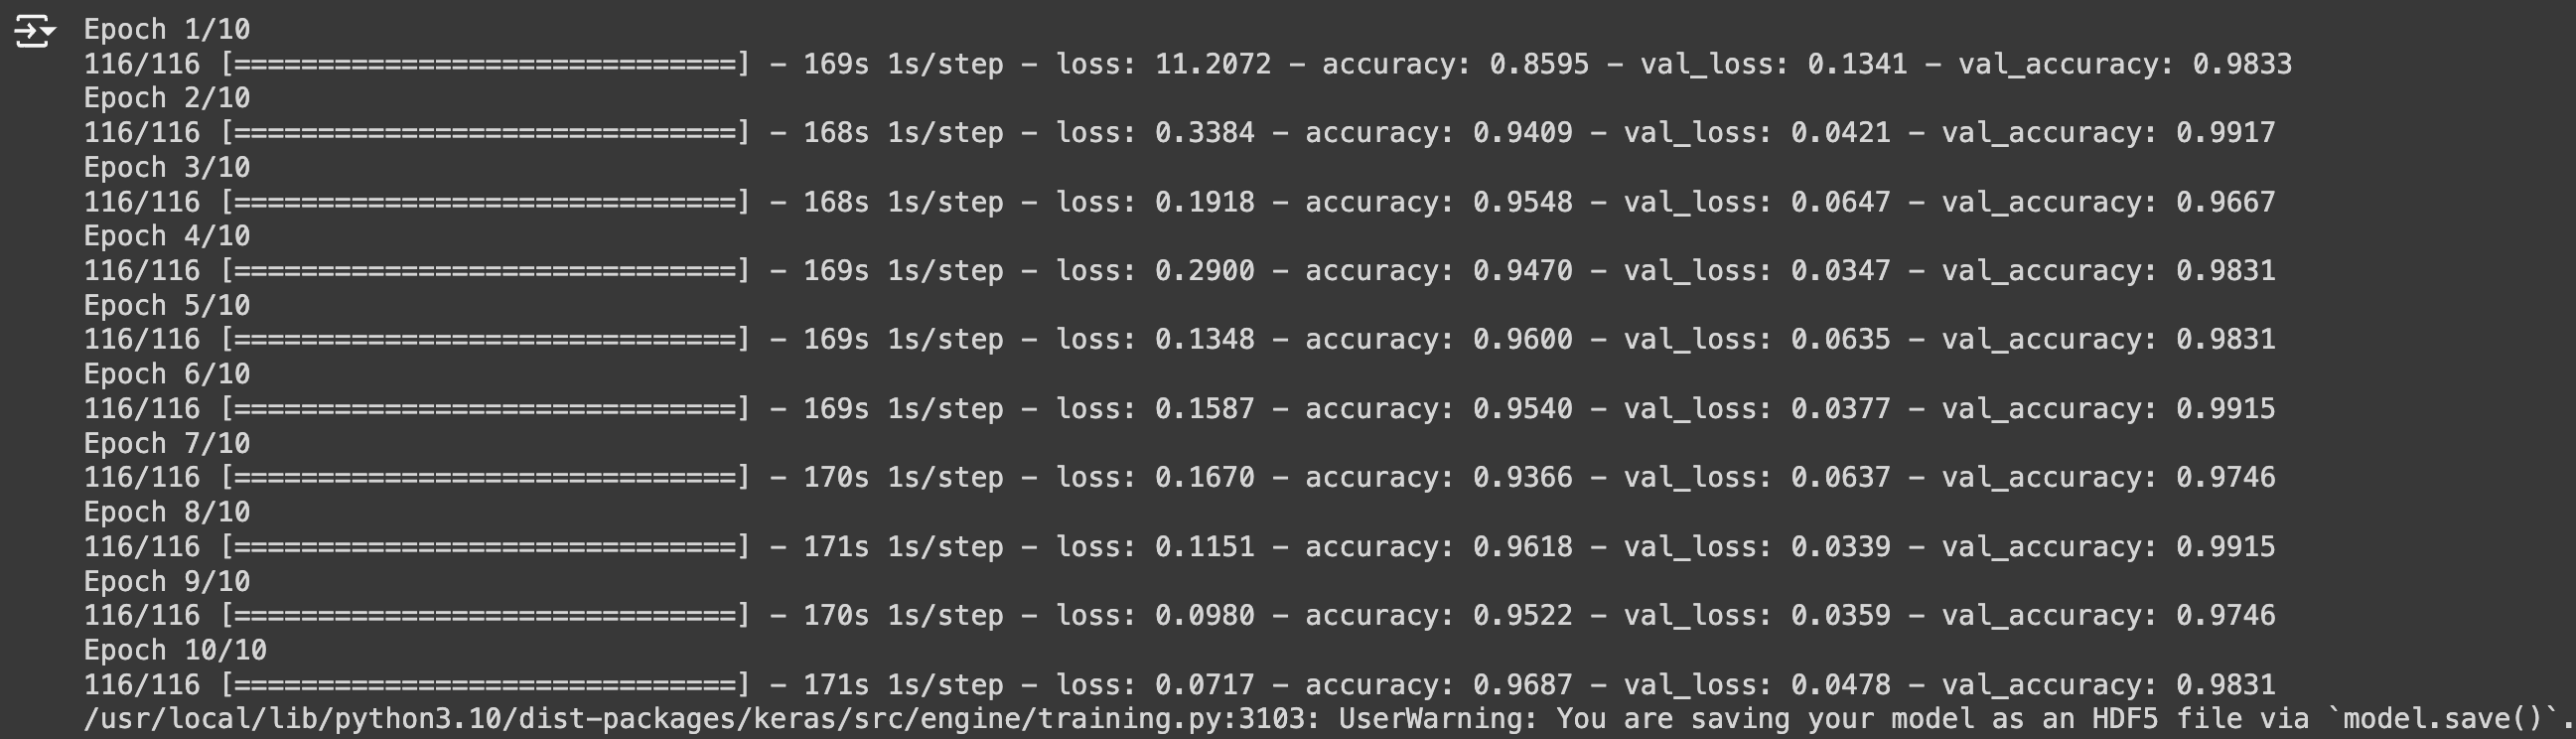
\includegraphics[width=\linewidth]{images/test-model.png}
    \caption{Model Test with original Dataset with training and validation accuracy and losses}
    \label{fig:test-model}
 \end{figure}

Since TensorFlow provides different Deep Learning (DL) models, every model has its own unique
density and layer count. For comparison purposes, all the hyperparameters were kept the same. 

\subsection{Evaluation of the Model}
On comparing the developed DICNN model with other state-of-art methods, the proposed model achieved good performance as depicted in the table \ref{tab:dicnn-comparison}.

\begin{table}[htbp]
    \centering
    \begin{adjustbox}{width=\textwidth}
    \begin{tabular}{llllll}
        \toprule
        \textbf{Ref} & \textbf{Category} & \textbf{Method} & \textbf{Dataset} & \textbf{Performance (\%)} & \textbf{XAI} \\
        \midrule
        \cite{Xu2022} & DL & Xception Network & 150,000 images & Acc: 83.99\% & No \\
        \cite{Fu2019} & DL & CNN & 60,000 images & Acc: 97.97\% & No \\
        \cite{Salman2022} & DL & dual-channel CNN & 9000 images & Acc: 100\% & No \\
        \cite{Zhang2017} & DL & CNN & 321,378 face images & Acc: 92\% & No \\
        \cite{Durall2019} & DL & Naive classifiers & Faces-HQ & Acc: 100\% & No \\
        \cite{Gandhi2020} & DL & VGG & 10,000 real and fake image & Acc: 99.9\% & No \\
        \cite{Gandhi2020} & DL & ResNet & 10,000 real and fake image & Acc: 94.75\% & No \\
        \cite{Yousaf2022} & DL & Two Stream CNN & 30,000 images & Acc: 88.80\% & No \\
        \cite{Hu2021} & Physical & Corneal specular highlight & 1000 images & Acc: 94\% & No \\
        \cite{Nightingale2021} & Human & Visual & 400 images & Acc: 50-60\% & No \\
        DICNN & DL & DICNN & 1289 images & Acc: 99.36 $\pm$ 0.62 & SHAP \\
        \bottomrule
    \end{tabular}
    \end{adjustbox}
    \caption{Comparison of model with other state-of-art methods}
    \label{tab:dicnn-comparison}
\end{table}

The model was validated with the original data used in the base research paper. The model was able to achieve the same level of accuracy as mentioned in the paper. The intention of the model was to gain the same accuracy as depicted in the base research paper, which was achieved. The result in depicted in the Figure. \ref{fig:test-model}.
\par After achieving the desired results, the model was then trained with different datasets to test the efficiency.

\subsection{Explainable AI (XAI)}
DL models are often considered as black-box models as they are complex and difficult to interpret. To make the model more interpretable, Explainable AI (XAI) is used. SHAP (SHapley Additive exPlanations) is a popular XAI technique. AI predicts and accepts results without explanation, this is where Explainable AI came into play. It gives clarification through analysis, masking, weight of features, maksing, numeric values and visualization.
The base model has incorporated SHAP, whereas in this research, the Local Interpretable Model-Agnostic Explanations (LIME) was used to explain the model in addition to SHAP as it can be used for DL models. It uses surrogate models to output the outcome. 

\end{section}

\pagebreak
